% **************************************************
% New Shapley Value Approximators -- Group Report
%
% Built on the chair's AIML thesis template (cleanthesis.sty), reduced to a report: the
% title page keeps the chair's layout but drops the reviewer block, and there is no
% declaration, acknowledgement or colophon.
% **************************************************
\documentclass[%
    paper=A4,
    twoside=false,          % a report is read on screen, not bound
    open=any,               % chapters may start on any page
    parskip=full,
    11pt,
    headings=normal,
    bibliography=totoc,
    listof=totoc,
    titlepage=on,
    captions=tableabove,
    chapterprefix=false,    % "1 Introduction", not "Chapter 1 / Introduction"
    numbers=noenddot,
    draft=false,
]{scrreprt}%  cleanthesis is built on a chapter-based class

% **************************************************
% Setup — adapted from the chair's my-thesis-setup.tex
%
% Kept: the chair's cleanthesis look and its package wiring. cleanthesis loads biblatex,
% hyperref, csquotes and listings itself, so they are configured through its options and
% \hypersetup rather than loaded again here.
%
% Dropped: everything only a thesis needs — reviewer/supervisor fields, title-page
% metadata, declaration, colophon.
% **************************************************

\PassOptionsToPackage{utf8}{inputenc}
\usepackage{inputenc}

% --------------------------
% Report metadata — edit these
% --------------------------
\newcommand{\reportTitle}{New Shapley Value Approximators}
\newcommand{\reportSubtitle}{Implementing LeverageSHAP, PolySHAP and OddSHAP in
    \texttt{shapiq}}
\newcommand{\reportSubject}{Praktikum Report}
\newcommand{\reportAuthors}{Group G \quad---\quad TODO: names}
\newcommand{\reportSupervisors}{TODO: supervisor names}
\newcommand{\reportDate}{\today}

\usepackage[english]{babel}

% --------------------------
% The chair's look. cleanthesis wires up biblatex, hyperref, csquotes and listings.
% --------------------------
\PassOptionsToPackage{%
    figuresep=colon,%
    hangfigurecaption=false,%
    hangsection=true,%
    hangsubsection=true,%
    sansserif=false,%
    configurelistings=true,%
    colorize=full,%
    colortheme=lmuaiml,%
    configurebiblatex=true,%
    bibsys=biber,%
    bibfile=references,%
    bibstyle=numeric-comp,%
    bibsorting=nyt,%
}{cleanthesis}
\usepackage{cleanthesis}
\ExecuteBibliographyOptions{backref=false, maxcitenames=2, maxbibnames=99, giveninits=true}

% cleanthesis sets BCOR=25mm, a binding correction for a printed and bound thesis. This
% report is read on screen and single-sided, so that 25mm is not swallowed by a binding --
% it just pushes every page to the right. Drop it and recompute the type area.
% DIV=12 is the thesis type area: a narrow block with wide margins to rest the eye over 60
% pages. A report is read in one sitting, so widen it. BCOR=25mm is a binding correction for
% a bound thesis; nothing binds this, and the 25mm only pushes every page right.
\KOMAoptions{BCOR=0mm, DIV=14}
\recalctypearea

% cleanthesis leaves 2.5 blank lines under every chapter heading and generous room around
% section headings. That is thesis pacing. Tighten it: five chapters do not need a page of
% air between them and their first sentence.
\renewcommand*\chapterheadendvskip{\vspace*{1.1\baselineskip}}
\RedeclareSectionCommand[beforeskip=-1.6ex plus -0.5ex, afterskip=0.9ex plus 0.2ex]{section}
\RedeclareSectionCommand[beforeskip=-1.2ex plus -0.4ex, afterskip=0.6ex plus 0.2ex]{subsection}
\RedeclareSectionCommand[beforeskip=-1ex plus -0.3ex, runin=true]{paragraph}

% cleanthesis leaves the head empty and puts the running mark and the page number in the
% footer. It redefines the footer for `plain` as well, but KOMA's own centred
% \cfoot{\pagemark} survives there, so every chapter-opening page -- which KOMA sets in
% `plain` -- printed its number twice, once from each. Use the same style throughout.
\renewcommand*{\chapterpagestyle}{scrheadings}

% --------------------------
% Maths, figures, tables
% --------------------------
\usepackage{mathtools}
\usepackage{amssymb}
\usepackage{float}% for [H] placement
\usepackage{subcaption}
\usepackage{booktabs}
\usepackage{tabularx}
% placeholder prose while the report is being written; every \lipsum is a paragraph
% somebody still has to write. Remove the package once they are all gone.
\usepackage{lipsum}

\hypersetup{%
    pdftitle={\reportTitle},
    pdfsubject={\reportSubject},
    pdfauthor={\reportAuthors},
}

% --------------------------
% Shorthands used across the report
% --------------------------
\newcommand{\shapiq}{\texttt{shapiq}}
\newcommand{\oddshap}{\mbox{OddSHAP}}
\newcommand{\leverageshap}{\mbox{LeverageSHAP}}
\newcommand{\polyshap}{\mbox{PolySHAP}}

% Every reproduction opens with one of these, so the reader sees what was run before
% reading any number. The three papers do not share a value function, so a configuration
% read after the results is a configuration read too late.
% Takes a short caption and a long one, like \caption[short]{long}: the long one carries the
% provenance, which belongs under the table, but a list of tables wants the short one.
%
% tabularx has to scan its whole body, so it cannot be split across this environment's begin
% and end. A p-column gives the same wrapping without that restriction.
\newenvironment{configtable}[2]{%
    \begin{table}[H]
    \centering
    \caption[#1]{#2}
    \begin{tabular}{@{}l p{0.72\textwidth}@{}}
    \toprule
}{%
    \bottomrule
    \end{tabular}
    \end{table}
}


\begin{document}

\renewcaptionname{english}{\figurename}{Fig.}
\renewcaptionname{english}{\tablename}{Tab.}

% --------------------------
% Front matter
% --------------------------
\pagenumbering{roman}
\pagestyle{empty}               % no number on the title page
% ==================================================
% Title page — the chair's layout, reduced to a report
%
% Taken from the template's content/titlepages.tex: same logos, same fonts, same
% colour. Dropped: the separate cover page, and the reviewer/supervisor block, which a
% report does not have.
% ==================================================
\begin{titlepage}
    \pdfbookmark[0]{Titlepage}{Titlepage}
    \tgherosfont
    \begin{figure}[t]
        \begin{minipage}[t]{8.5cm}
            
\includegraphics[height=1.8cm,width=3.6cm]{gfx/lmulogo.pdf}\\
            \textsf{\small{Department of Mathematics, \\ Informatics and Statistics \\
                Institute of Informatics}}
        \end{minipage}
        \hfill
        \begin{minipage}[t]{4.7cm}
            
\includegraphics[height=1.8cm,width=4.7cm]{gfx/aiml-logo-solid-black.pdf}\\
            \textsf{\hspace*{0.1cm}\small{Artificial Intelligence and \\
                \hspace*{0.1cm}Machine Learning}}
        \end{minipage}
    \end{figure}

    \centering
    \vfill
    {\large \reportSubject} \\[5mm]
    {\LARGE \color{ctcolortitle}\textbf{\reportTitle}} \\[6mm]
    {\large \reportSubtitle} \\[10mm]
    {\Large \reportAuthors} \\
    \vfill

    % Names only: the logos above already give the department and the group, so repeating
    % the affiliation here says nothing and forces an ugly hyphenation.
    \begin{minipage}[t]{.27\textwidth}
        \raggedleft
        \textit{Supervisors}
    \end{minipage}
    \hspace*{15pt}
    \begin{minipage}[t]{.65\textwidth}
        {\Large \reportSupervisors}
    \end{minipage}

    \vfill
    {\large \reportDate}
    \vspace*{10mm}
\end{titlepage}


\pagestyle{plain}               % page number only, no running head
\currentpdfbookmark{\contentsname}{toc}
\setcounter{tocdepth}{1}        % chapters and sections; the report is 5 chapters deep
\tableofcontents
\clearpage

% --------------------------
% Body
% --------------------------
\pagenumbering{arabic}
\setcounter{page}{1}
\pagestyle{scrheadings}         % cleanthesis puts the number in the running head; without
                                % this, KOMA also prints one in the footer and every page
                                % carries it twice

% ==================================================
% 1. Abstract and introduction
%
% Deliberately no numbered subsections: cleanthesis section headings are tall, and an
% introduction this short does not need a table of contents of its own. Paragraph breaks
% carry the structure instead.
% ==================================================
\chapter{Abstract and Introduction}
\label{sec:introduction}

\section*{Abstract}

We add three recent Shapley-value approximators to \shapiq{} --- \leverageshap{}
\citep{Witter.2025a}, \polyshap{} \citep{Fumagalli.2026a} and \oddshap{}
\citep{Fumagalli.2026} --- reproduce each paper from the resulting implementation, and
benchmark all three against every approximator \shapiq{} already provides on one shared
testbed. Each paper's headline claim holds, and holds on a value function none of the three
papers uses: \oddshap{} leads on the high-dimensional games once the budget passes the
threshold its paper predicts, \leverageshap{} beats optimised KernelSHAP at every dimension,
and \polyshap{} is strongest at low dimension and degrades at high, for the reason its own
paper gives. The comparison also shows that no single ordering of the three exists. Averaged
over all games \leverageshap{} ranks best; restricted to the games above sixty players
\oddshap{} does, by a wide margin. Which of those two numbers is the answer depends on the
dimension a reader cares about, and reporting either alone would misrepresent the other.

% --------------------------------------------------
% The introduction runs as continuous prose. Roughly one paragraph per block.
% --------------------------------------------------

\paragraph{What this report is.}
The Shapley value assigns each feature its average marginal contribution over all $2^d$
coalitions, which is why every practical use of it rests on an approximator. This report covers
three recent ones. We implemented each in \shapiq{} \citep{Muschalik.2024b}, reproduced the
experiments of the paper that introduced it, and then compared all three against the
approximators \shapiq{} already had. Chapter~\ref{sec:benchmark} is the comparison that puts
every method on the same footing; Chapters~\ref{sec:oddshap} to~\ref{sec:polyshap} take each
approximator on its own terms, first summarising its paper, then reproducing it.

\paragraph{What we did.}
Three approximators were implemented and submitted upstream. \oddshap{} is merged
(PR~\#522, with a follow-up in PR~\#560); \leverageshap{} (PR~\#524) and \polyshap{}
(PR~\#559) are open at the time of writing. Each has a reproduction of its paper, driven by
committed result tables so that every figure re-renders offline in minutes, without a GPU and
without re-running the experiments. On top of those, the cross-method benchmark of
Chapter~\ref{sec:benchmark} runs every approximator registered in \shapiq{} over a shared set
of eleven games, twelve budgets and ten explained predictions --- 19{,}800 cells in total.
Two defects in \shapiq{} surfaced while the benchmark was being built and are fixed alongside
this work: the ViT value function moved its model to the GPU but left its normalisation
parameters on the CPU, so it could not run there at all; and the placeholder classes that stand
in for the optional \texttt{sparse} and \texttt{shapleig} extras were abstract, so a missing
dependency was reported as a broken approximator rather than as a missing dependency.

\paragraph{How to read it, and one distinction that runs through it.}
The report answers two different questions, and they need different setups. A
\emph{reproduction} asks whether a paper's claim survives re-implementation; it has to use that
paper's own value function, or it tests nothing. The three papers do not share one --- \oddshap{}
alone trains XGBoost classifiers and defines its tabular value function by interventional
perturbation over fifty background instances. The \emph{benchmark} asks how the methods compare
with each other and with what \shapiq{} already had; it has to use a single value function for
every method, which then belongs to no paper in particular. The consequence is worth stating
before any table is read: the absolute errors in Chapter~\ref{sec:benchmark} and those in
Chapters~\ref{sec:oddshap} to~\ref{sec:polyshap} are different quantities, measured against
different targets, and comparing them across chapters is meaningless. Within each chapter they
are directly comparable, which is what each chapter is for. That the papers' claims survive the
move to a value function none of them chose is the stronger result, and it is only visible
because the two settings are kept apart.

% ==================================================
% 2. Cross-method benchmark
%
% Every number here is computed from
%   benchmark/results/lmu_full_sweep_20260717/results.csv
% whose README records the command, the code revision and the machine.
% Task packet: plan/task-packets/02-benchmark.md
% ==================================================
\chapter{Cross-Method Benchmark}
\label{sec:benchmark}

\section{Setup}
\label{sec:benchmark:setup}

\begin{configtable}{Benchmark configuration}{Benchmark configuration. Provenance:
    \texttt{benchmark/results/lmu\_full\_sweep\_20260717/README.md}.}
    Games & 11 --- SOUM($n$=6,8,10) and the ML games IRIS(4), California(8), Diabetes(10),
        Adult(12), Correlated(60), Independent(60), NHANES(79), Communities(101). The ML
        grid follows Musco \& Witter. \\
    Value function & Features masked against a single baseline row (the training mean);
        \texttt{XGBRegressor}, 100 trees, depth 4. \emph{Not} any paper's value function
        --- see Chapter~\ref{sec:introduction}. \\
    Ground truth & Exact enumeration for $n \le 10$; interventional TreeSHAP against the
        same baseline row above it. \\
    Budgets & $m = c \cdot n$ for $c \in \{1,2,3,5,8,12,20,30,50,75,110,160\}$. \\
    Repeats & 10 held-out predictions per game, model fixed. Median and IQR are over
        those predictions. \\
    Methods & Every approximator registered in
        \texttt{shapiq.approximator.SV\_APPROXIMATORS} (15 registered, 14 ran). \\
    Scale & 19{,}800 cells, 143{,}980 metric rows, run on the LMU CIP cluster. \\
\end{configtable}

Two choices in that table shape everything that follows. The first is that budgets are multiples
of the number of players rather than fractions of the coalition space. A fraction of $2^n$ stops
being a runnable budget once $n$ grows --- on Independent($n$=60) even five percent of the space is
$5.8 \times 10^{16}$ evaluations --- and at the other end a budget equal to $2^n$ makes every
method exact, so ranks there record ties rather than a comparison. Multiples of $n$ are the
convention the approximator papers use, they apply to every game in the grid, and they place the
large games in the under-determined regime where the methods actually differ.

The second is that a repeat explains one held-out prediction of one fixed model. Had each repeat
retrained the model, the spread across repeats would have mixed estimator noise with model noise
and could have been read as neither: a different tree has different Shapley values, so the target
would move with the repeat. Fixing the model makes the band the spread across predictions, which
is what the approximator papers report and what a reader assumes an error band to be.

\section{Results and Discussion}
\label{sec:benchmark:results}

Averaged over all eleven games, \leverageshap{} takes the best mean rank at $3.24$, just ahead of
\oddshap{} at $3.31$, with \polyshap{} at $4.50$, OptimizedKernelSHAP at $4.69$ and RegressionMSR
at $5.46$. Reading that as a verdict would be a mistake, and the same data says why: over those
cells \oddshap{} wins outright $652$ times against \leverageshap{}'s $168$. A method that comes
first four times as often cannot also be the one that is, on average, slightly worse --- unless the
average is carried by cells in which coming first means very little.

That is what is happening. Splitting the games by dimension inverts the ordering. On the seven
small games ($n \le 12$, 840 comparison cells) \leverageshap{} leads at $3.55$, \polyshap{} follows
at $3.68$, and \oddshap{} is third at $4.51$. On the four large games ($n \ge 60$, 480 cells)
\oddshap{} leads at $1.34$, \leverageshap{} is second at $2.69$, and the best baseline,
OptimizedKernelSHAP, is far behind at $4.58$. The aggregate is not a compromise between the two
regimes; it is dominated by the first, which contributes almost twice as many cells.

The inversion is not noise but saturation. Among the small-game results $24.0\%$ are already exact
to machine precision, taking MSE below $10^{-10}$ as the threshold; among the large-game results
only $1.0\%$ are. Figure~\ref{fig:benchmark:soum} shows what that looks like: on SOUM($n$=10) every
method collapses to the numerical floor as the budget approaches $2^{10}$, and what happens to the
left of that collapse decides a rank that the collapse then erases. Where a quarter of the results
are exact, a rank is a tie-break rather than a measurement. The large games, where almost nothing
is exact, carry the comparison.

\begin{figure}[H]
    \centering
    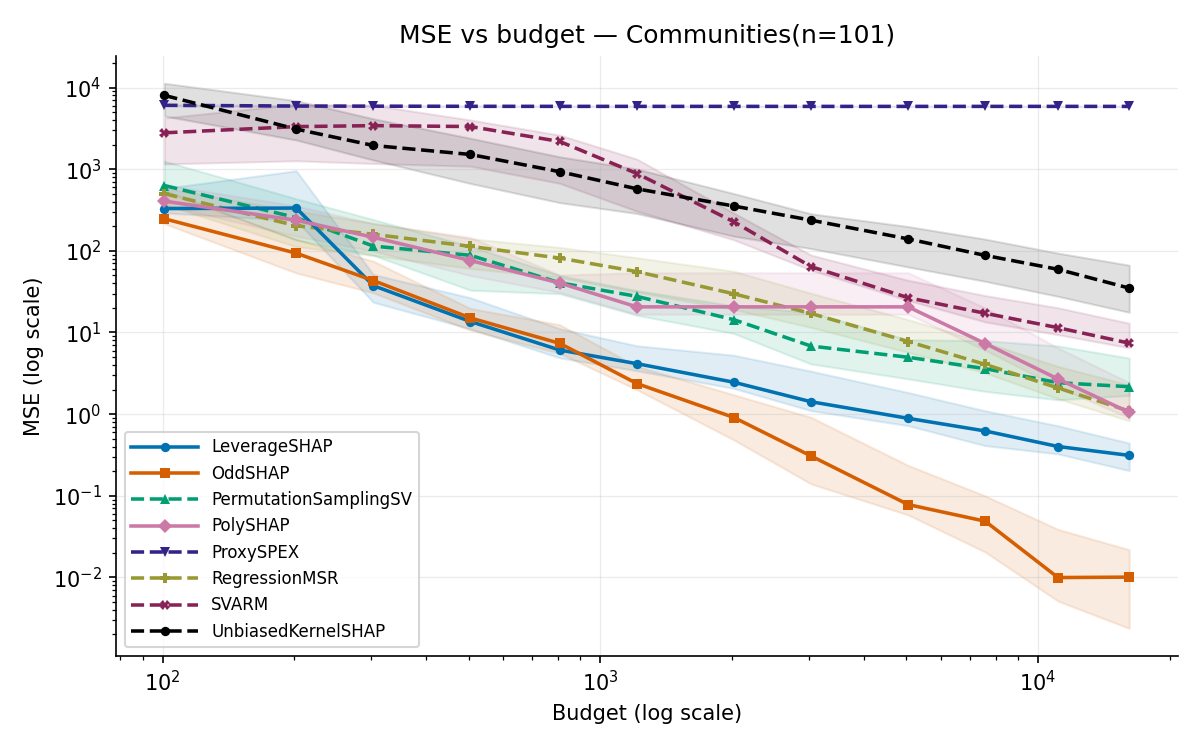
\includegraphics[width=\textwidth]{figures/bench-communities-n101.png}
    \caption[MSE against budget on Communities ($n=101$)]{MSE against budget on Communities
        ($n=101$), the largest game in the grid. Median over the ten explained predictions; the
        band is the interquartile range across them. Solid curves are the approximators added in
        this project, dashed are baselines. \oddshap{} separates from the field at roughly
        $m = 500 \approx 5d$ and ends about an order of magnitude below the runner-up.}
    \label{fig:benchmark:communities}
\end{figure}

The two regimes are not a ranking of the three methods but a division of labour between them, and
each half is what the method's own paper says it should be. Taken in turn:

\polyshap{} is second on the small games at $3.68$ and sixth on the large ones at $5.94$, the
largest swing of the three. \citet{Fumagalli.2026a} claims exactly the near half of that: in
low-dimensional settings its order-3 variant "yields the best performance" on the paper's tabular
datasets. It also states the mechanism that closes the far half --- the support is every
interaction up to a fixed order $k$, which costs $O(d^k)$ terms, so higher orders "require a
larger sampling budget". At $d = 101$ that support is unaffordable at any budget in our grid, and
the method degrades to the field. Its regime is real and it is narrow.

\leverageshap{} is the most uniform of the three: first on the small games at $3.55$ and second on
the large at $2.69$, never far from the top. \citet{Witter.2025a} makes a narrower claim than a
leaderboard position --- that leverage-score sampling "can even outperform the highly optimized
Kernel SHAP\ldots, especially for large $n$" --- and that claim is about a specific opponent, which
is in our grid. It holds, including the qualifier: \leverageshap{} leads OptimizedKernelSHAP by
$1.20$ ranks on the small games and by $1.89$ on the large ones. The advantage does not merely
survive the move to high dimension, it grows there, which is what an $O(n \log n)$ sampling
guarantee predicts against a heuristic.

\oddshap{} inverts \polyshap{}: third on the small games at $4.51$, first on the large at $1.34$,
and the gap to the runner-up is a rank and a third. On the large games its advantage also switches
on at a predictable budget. Ranking it within each budget separately gives $3.40$ at $m = d$, where
plain stratified sampling beats it; $1.35$ at $2d$; $1.30$ at $5d$; and then $1.00$, $1.00$,
$1.02$, $1.00$, $1.07$, $1.00$ and $1.05$ at $12d$ through $160d$. From twelve times the dimension
onward it is first in essentially every cell. Its interaction factor is $\eta = 10$, so the
threshold is $m > \eta d$ --- the condition \citet{Fumagalli.2026} attaches to its own claim.
Below it the screening cannot pay for itself; above it the method has an adaptive support where
\polyshap{} has a fixed one, which is why the two occupy opposite ends of the dimension axis. The
runner-up above the threshold is always \leverageshap{}, drifting from $2.05$ at $12d$ to $2.65$ at
$160d$: that gap widens with budget instead of closing, which is what one expects if two methods
differ in what they can represent rather than in how quickly they converge.

One deviation is worth stating rather than smoothing. \citet{Fumagalli.2026} reports that at low
dimension \oddshap{} performs *like* RegressionMSR; on our small games it is ahead of it, $4.51$
against $5.62$. Our small games are smaller than the paper's low-dimensional value functions
($n \le 12$ against $d = 14$ to $16$), and the value function is not the paper's, so the two
statements are not in contradiction --- but they are not the same statement either.

None of this reproduces or refutes anything, and the reason is in the configuration table. Each
paper defines its own value function: \citet{Fumagalli.2026} trains XGBoost classifiers and
perturbs interventionally over fifty background instances; \citet{Fumagalli.2026a} trains random
forests and perturbs path-dependently; \citet{Witter.2025a} uses tree models whose exact values
TreeSHAP can supply. This benchmark uses none of the three. What it offers instead is a
cross-check: three claims, each made under its own conditions, each still visible under a fourth
set of conditions that belongs to nobody. That is weaker than a reproduction in what it licenses
--- it cannot confirm a number --- and stronger in what it suggests, since a regime that survives a
change of value function is more likely to be a property of the method than of the setup. The MSE
magnitudes here therefore cannot be compared with those in
Chapters~\ref{sec:oddshap}--\ref{sec:polyshap}, only the orderings.

The orderings, at least, do not depend on the metric. Repeating the comparison under the relative
$\ell_2$ error that \citet{Witter.2025a} reports rather than MSE leaves both regimes intact:
\leverageshap{} first on the small games at $3.64$ ahead of \polyshap{} at $3.77$, \oddshap{} first
on the large at $1.71$ ahead of \leverageshap{} at $3.22$.

\begin{figure}[H]
    \centering
    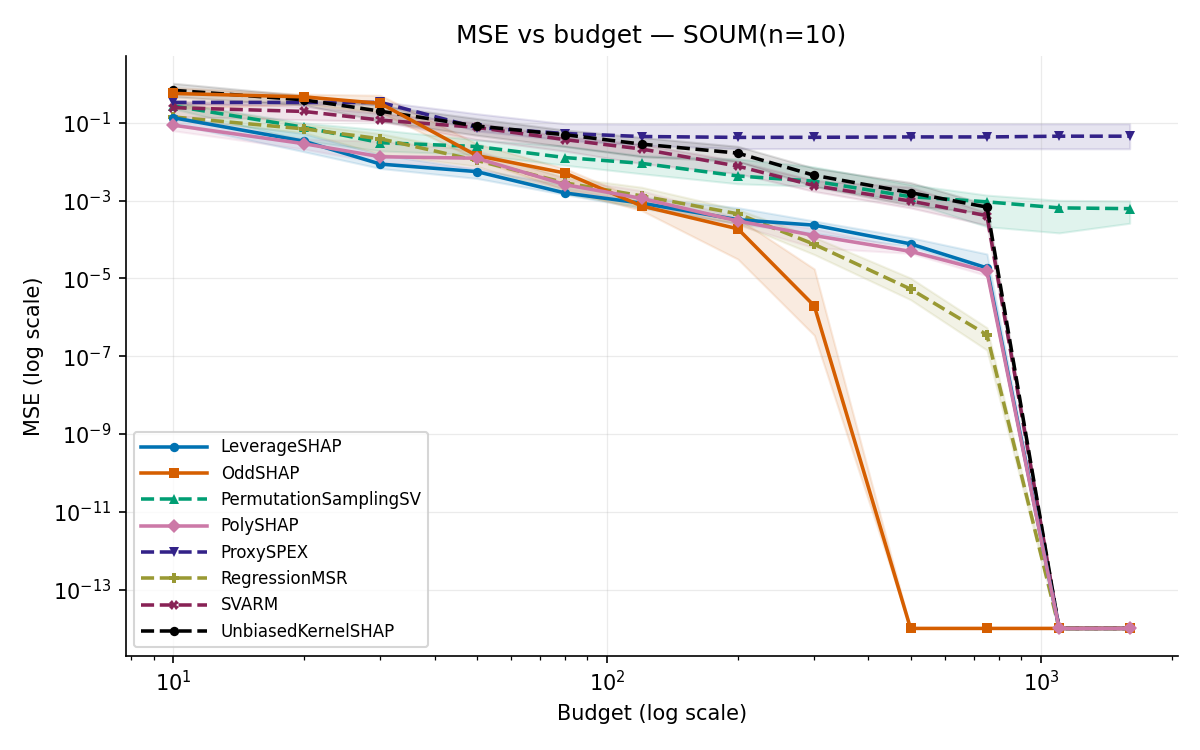
\includegraphics[width=\textwidth]{figures/bench-soum-n10.png}
    \caption[MSE against budget on SOUM ($n=10$)]{MSE against budget on SOUM ($n=10$), a small
        game. Every method falls to the numerical floor as the budget approaches full enumeration
        ($2^{10} = 1024$); $24\%$ of all small-game results are exact in this sense. Ranks in that
        region are tie-breaking rather than comparison, which is why the aggregate over all eleven
        games should not be read as a verdict.}
    \label{fig:benchmark:soum}
\end{figure}

\paragraph{Threats to validity.}
The value function is not any paper's, so this chapter compares the methods with each other and
does not test any paper's claim; that is what Chapters~\ref{sec:oddshap}--\ref{sec:polyshap} are
for. Coverage is uneven, and average ranks across methods that ran in different numbers of cells
are not directly comparable, because a method that declines a budget is scored only where it ran.
\oddshap{} declines 50 cells, all at $m = d$ or $2d$ on the four smallest games, where the budget
falls below its minimum of $\eta = 10$ evaluations; it declines none on the large games, where it
ran in all 480. SPEX declines 680 cells and ProxySPEX 10. ShaplEIG is registered but needs an
optional extra that was not installed, so it is skipped in all 1{,}320 of its cells and appears in
no figure. Ten predictions per game make the quartiles a coarse envelope rather than a confidence
interval. Finally, FourierSHAP and the fixed-budget FFD variants belong to
\citet{Fumagalli.2026}'s own comparison but are not implemented in \shapiq{}, so the baselines
here are that paper's set intersected with what was available, not the set in full.

% ==================================================
% 3. OddSHAP
% ==================================================
\chapter{OddSHAP}
\label{sec:oddshap}

\section{Summary}
\label{sec:oddshap:summary}

% Written by Sara; adapted from oddshap_summary.md, converted to LaTeX.

\paragraph{The core idea.}
Every set function $f: 2^{[d]} \to \mathbb{R}$ splits into an odd and an even part,
$f = f_{\mathrm{odd}} + f_{\mathrm{even}}$, where
$f_{\mathrm{odd}}(S) = \tfrac{1}{2}\left(f(S) - f(S^{c})\right)$ and
$f_{\mathrm{even}}(S) = \tfrac{1}{2}\left(f(S) + f(S^{c})\right)$. The paper's key observation
(Observation~3.1) is that the Shapley value depends only on $f_{\mathrm{odd}}$:
$\phi_i(f) = \phi_i(f_{\mathrm{odd}})$ for every player $i$. The marginal contributions of
complementary coalitions cancel the even part out when summed over all subsets.

This explains why paired sampling --- evaluating $S$ and $S^{c}$ together --- helps as much as
it does in practice. The authors show (Theorem~3.2) that under paired samples a regression
objective over a function class closed under the odd/even decomposition splits into two
independent problems, one per part. Since only the odd part matters for $\phi_i$, paired
sampling implicitly filters out irrelevant even structure. It also motivates the estimator
itself: if only $f_{\mathrm{odd}}$ has to be recovered, no budget should be spent fitting
even-order terms at all.

\paragraph{Why the Fourier basis.}
The usual regression estimators (KernelSHAP, \leverageshap{}, \polyshap{}) work in the
unanimity/Möbius basis, whose basis functions mix odd and even components. The Fourier (Walsh)
basis $\chi_T(S) = (-1)^{|S \cap T|}$ does not: $\chi_T$ is an odd function exactly when $|T|$
is odd. The authors therefore restrict a Fourier regression to odd-cardinality terms, and show
(Theorem~3.5) that the constrained regression is still consistent --- it recovers the Shapley
values through the same projection KernelSHAP and \polyshap{} use.

\paragraph{The estimator.}
Algorithm~1 has three steps.
\begin{enumerate}
    \item \textbf{Paired sampling.} Coalitions are drawn without replacement, uniformly over
        coalition sizes, and every sampled $S$ is paired with its complement $S^{c}$.
    \item \textbf{Interaction screening.} A gradient-boosted tree is fit to the sampled
        coalitions and converted to its Fourier spectrum; the odd-cardinality terms with the
        largest coefficients are kept as candidates. The candidate budget is
        $\lceil m/\eta \rceil$, where $\eta$ trades support size against regression budget.
        The paper's default is $\eta = 10$.
    \item \textbf{Sparse odd regression.} A weighted least-squares problem is solved over the
        singletons plus the selected higher-order odd terms, with the empty and full coalition
        values as exact boundary constraints --- efficiency is enforced, not approximated by
        large weights. The Shapley values follow in closed form as
        $\phi_i = -2 \sum_{T \ni i,\, |T| \text{ odd}} \beta_T / |T|$.
\end{enumerate}
If the budget cannot cover even the linear terms ($m < d\eta$), the paper falls back to reading
the Shapley values off the fitted tree with TreeSHAP.

\paragraph{What the paper reports.}
The paper benchmarks eight value functions --- DistilBERT and ViT-16 from \shapiq{}, plus
tabular XGBoost and synthetic games up to $d = 101$ --- against Permutation Sampling, SVARM,
MSR, \leverageshap{}, \polyshap{} and RegressionMSR, measuring MSE against budget $m$ (Figure~2)
and against wall-clock runtime under simulated evaluation costs (Figure~3). \oddshap{} attains
the best average rank overall (1.50, Table~1) and wins clearly once $m > \eta d$; at very low
budgets it degrades to the tree fallback and performs comparably to RegressionMSR and
\leverageshap{}. An ablation (Figure~4) shows that adding up to roughly 1{,}000 odd interactions
gives a 6--62$\times$ MSE reduction over the interaction-free baseline, but that too many
interactions eventually overfit and reverse the gain --- which is why the candidate budget is
capped at $\lceil m/\eta \rceil$ rather than enumerated.

\section{Reproduction and Discussion}
\label{sec:oddshap:reproduction}

% The configuration comes first, deliberately: the paper's value function is not the benchmark's
% of Chapter~\ref{sec:benchmark}, and a reader who assumes otherwise misreads every number
% below. The entries are taken from the paper, Section 5.

\begin{configtable}{\oddshap{} reproduction configuration}{Configuration of the \oddshap{} reproduction, following
    \citet{Fumagalli.2026}. Provenance: \texttt{notebooks/oddshap/README.md}.}
    Value functions & 8 --- tabular: Cancer ($d$=30), Estate ($d$=15), CG60 ($d$=60),
        IL60 ($d$=60), NHANES ($d$=79), Crime ($d$=101); deep learning: ViT-16 ($d$=16),
        DistilBERT ($d$=14). \\
    Model (tabular) & XGBoost \emph{classifier}; continuous targets binarised at the
        median. \\
    Value function (tabular) & Interventional feature perturbation, estimated from
        \textbf{50 background instances}. \\
    Ground truth (tabular) & Interventional TreeSHAP. \\
    Value function (deep) & Baseline imputation; ground truth by exhaustive summation. \\
    Budgets & $m$ from $d+1$ to $\min(2^d,\,20\,000)$, sampled uniformly over coalition
        sizes. \\
    Repeats & 30 randomly selected predictions per value function; median and IQR are taken
        across them. \\
    Baselines & 6 --- KernelSHAP, MSR, PermSamp, RegressionMSR, SVARM, kADDSHAP. \\
    Variants & \texttt{v522\_merged} (as merged, PR~\#522) and \texttt{v560\_improved}
        (the follow-up, PR~\#560). \\
    Deviation & No TreeSHAP fallback below $m < d\eta$: an under-budgeted call raises
        \texttt{ValueError} rather than returning another estimator's values. \\
\end{configtable}

The configuration above is the paper's, not the benchmark's of Chapter~\ref{sec:benchmark}. The
two differ in every respect that sets the scale of the error: a classifier against a regressor,
an interventional value function over 50 background instances against masking to a single
baseline row, interventional TreeSHAP against exact enumeration. The MSE values in this chapter
and in Chapter~\ref{sec:benchmark} are therefore different quantities, and are not comparable.

\paragraph{Deviation from the paper.}
The paper falls back to TreeSHAP on the fitted tree whenever $m < d\eta$. This implementation
deliberately does not: an under-budgeted call to \oddshap{} should not silently return a
different estimator's values. The minimum usable budget is lowered to $\eta$ instead, and below
it the call raises \texttt{ValueError}, unless the budget already covers the full coalition
space ($m \geq 2^{d}$). The reproduction therefore does not cover the low-budget,
high-dimension regime of the paper's Figure~2, and may diverge from the paper there.

\paragraph{Results.}
% Verified against the committed CSVs in notebooks/oddshap/data/.
\oddshap{} takes rank~1 on 7 of the 8 value functions, averaging 1.125, and both variants agree on
every one (Table~\ref{tab:oddshap:ranks}). The exception is DistilBERT, the lowest-dimensional
value function, where RegressionMSR wins --- which is what the paper itself reports for its
low-dimensional cases, stating that \oddshap{} performs on par with RegressionMSR rather than ahead
of it. The claimed ordering reproduces, including the exception the paper predicts.

\begin{table}[H]
    \centering
    \caption[\oddshap{} rank per value function]{\oddshap{}'s rank on each value function, both
        variants, from the committed CSVs. Rank~1 on 7 of 8; the sole exception is the smallest
        $d$, where the paper also expects parity rather than a win.}
    \label{tab:oddshap:ranks}
    \begin{tabular}{@{}lcccccccc@{}}
        \toprule
        & \multicolumn{6}{c}{tabular} & \multicolumn{2}{c}{deep} \\
        \cmidrule(lr){2-7}\cmidrule(lr){8-9}
        & Crime & NHANES & CG60 & IL60 & Cancer & Estate & ViT-16 & DistilBERT \\
        $d$ & 101 & 79 & 60 & 60 & 30 & 15 & 16 & 14 \\
        \midrule
        PR~\#522 & 1 & 1 & 1 & 1 & 1 & 1 & 1 & \textbf{2} \\
        PR~\#560 & 1 & 1 & 1 & 1 & 1 & 1 & 1 & \textbf{2} \\
        \bottomrule
    \end{tabular}
\end{table}

The accuracy advantage appears with budget as the paper describes, and the reproduced curves track
the published ones over three orders of magnitude (Figure~\ref{fig:oddshap:fig2}).

The interaction ablation reproduces on every value function, non-monotonicity included
(Figure~\ref{fig:oddshap:fig4}): the MSE ratio drops as odd interactions are added, bottoms out
around $\eta = 10$ to $5$, then rises \emph{above} 1 at $\eta = 2$, where the support is large
enough to overfit and the estimate is worse than using no interactions at all. That is the paper's
argument for capping the candidate budget instead of enumerating. The trough depth differs --- ours
reaches further below 1 on Cancer than the paper's does --- so the reproduction supports the shape
of the claim rather than its magnitude.

\begin{figure}[tbp]
    \centering
    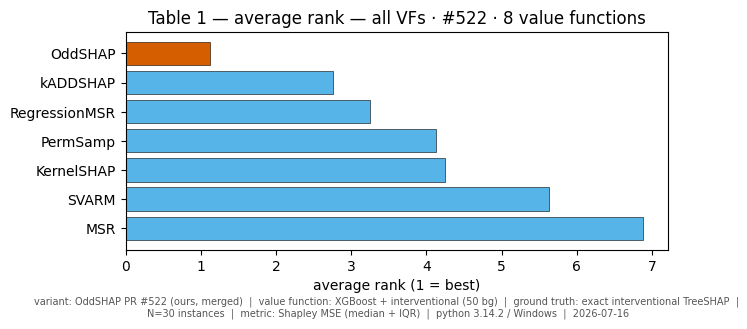
\includegraphics[width=0.86\textwidth]{figures/oddshap-rank-table.png}
    \caption[Average rank across the eight value functions]{%
        \textbf{Average rank} (the paper's Table~1), PR~\#522. Lower is better; rank~1 is the
        lowest median MSE on a value function. \oddshap{} averages 1.125 over the six baselines
        shown --- not comparable with the paper's 1.50, see below.}
    \label{fig:oddshap:rank}
\end{figure}

\begin{figure}[tbp]
    \centering
    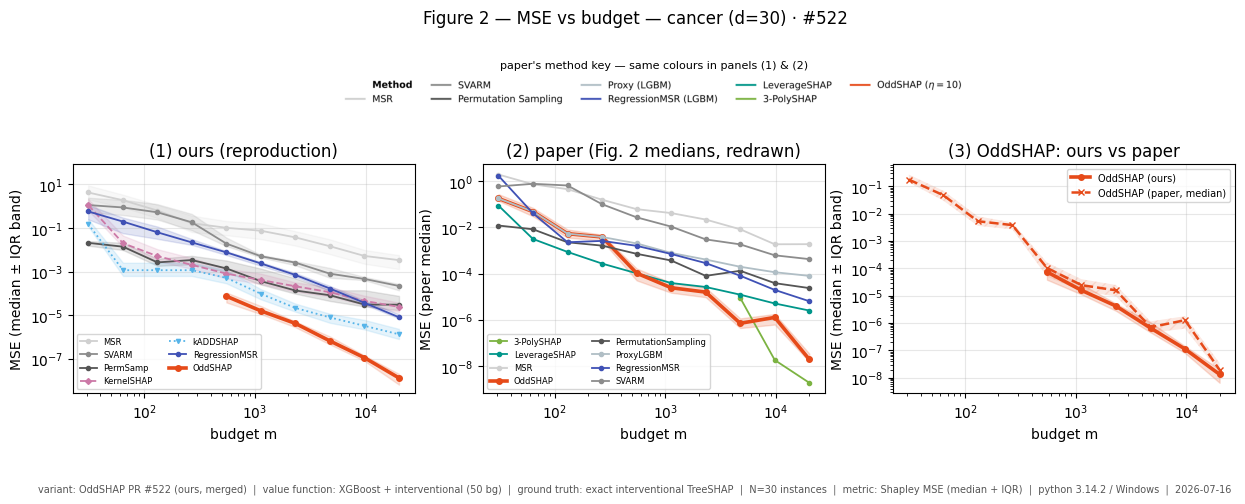
\includegraphics[width=\textwidth]{figures/oddshap-fig2-first.png}
    \caption[MSE against budget, ours against the paper's]{%
        \textbf{MSE against budget on Cancer ($d=30$)}, reproducing the paper's Figure~2.
        Log--log; median over 30 predictions, band is the IQR.
        \textbf{(1)} ours, against \shapiq{}'s six baselines. \textbf{(2)} the paper's medians,
        redrawn --- a different method set, hence not a like-for-like overlay.
        \textbf{(3)} \oddshap{} alone: ours (solid) against the paper's digitised median
        (dashed).}
    \label{fig:oddshap:fig2}
\end{figure}

\begin{figure}[tbp]
    \centering
    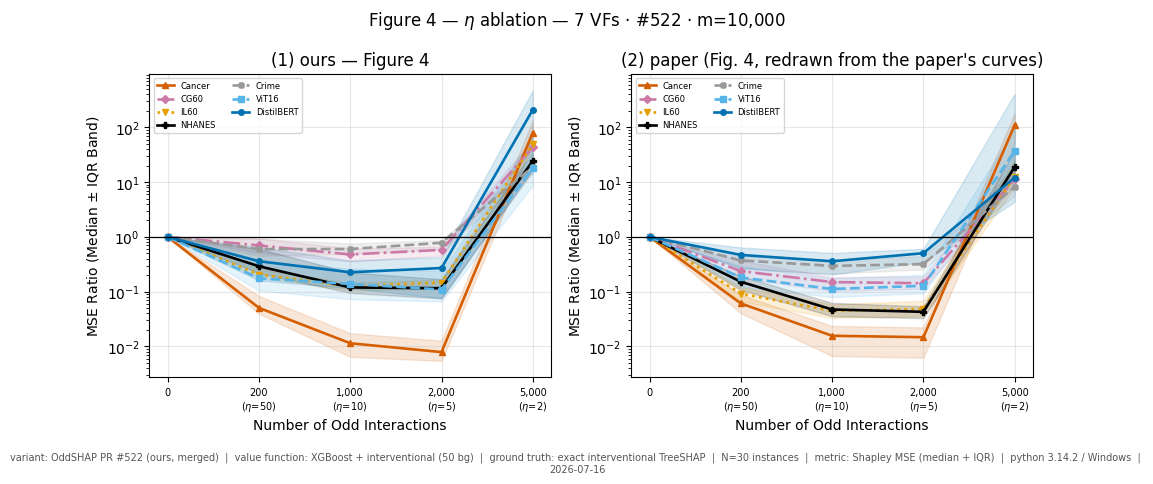
\includegraphics[width=\textwidth]{figures/oddshap-fig4-eta.png}
    \caption[The interaction ablation]{%
        \textbf{The interaction ablation} (the paper's Figure~4) at $m = 10{,}000$, seven value
        functions --- Estate excluded, as the paper excludes it. $y$: MSE \emph{ratio} against
        the interaction-free baseline, so $1.0$ means the interactions changed nothing.
        $x$: odd interactions admitted, fixed by $\lceil m/\eta \rceil$; the annotated $\eta$
        runs from 50 (few) to 2 (many). \textbf{(1)} ours, \textbf{(2)} the paper's, redrawn.}
    \label{fig:oddshap:fig4}
\end{figure}

\paragraph{Reading the average rank.}
Our 1.125 should not be read against the paper's 1.50 as an improvement. The two averages are
taken over different baseline pools: ours over the six baselines in the configuration table,
the paper's over a larger set that also includes \leverageshap{}, \polyshap{}, FourierSHAP and
the fixed-budget FFD variants. A smaller pool makes rank~1 easier to hold. The number
reproduces the \emph{ordering}, not the value.

\paragraph{The two variants.}
PR~\#560 relaxes the minimum budget from $n\eta$ to $\eta$ and merges paired regression rows.
Above the minimum budget the two agree to machine precision --- the largest relative deviation
across the tabular value functions is of order $10^{-12}$, and on the two deep-learning value
functions they agree bitwise. Every paper-scale result is therefore unchanged by the follow-up;
its entire effect is confined to the low-budget regime in which PR~\#522 refuses.

\paragraph{Honest gaps.}
The two deep-learning value functions are budget-truncated: ViT-16 reaches a budget of 1{,}895
and DistilBERT 1{,}591, rather than the paper's sweep to $\min(2^d, 20\,000)$. Both are
low-dimensional ($d = 16$, $d = 14$) --- the regime in which the paper itself reports
convergence between the methods --- and the $\eta$ ablation is complete for both. The
high-budget tail for these two is nevertheless not confirmed here. Separately, the reference
curves in
\texttt{paper\_reference/} are digitised from the published figures rather than taken from
author-provided numbers, and are accurate only to the resolution of that source.

% ==================================================
% 4. LeverageSHAP
% ==================================================
\chapter{LeverageSHAP}
\label{sec:leverageshap}

% Owner: TODO (LeverageSHAP was contributed by a teammate; this section is theirs to
% write). The structure mirrors Section~\ref{sec:oddshap} so the three read alike.

\section{Summary}
\label{sec:leverageshap:summary}

% TODO. What the paper does \citep{Witter.2025}. A one-page summary already exists as
% notebooks/leverageshap_discussion/leverageshap_summary.pdf -- reuse it.
% Worth covering:
%   - the core idea: leverage-score sampling for the KernelSHAP regression, and why that
%     is the right sampling distribution;
%   - how it relates to the others: the OddSHAP paper describes LeverageSHAP as
%     "OddSHAP without interactions", which is a useful anchor for the reader;
%   - the constrained solve, rather than KernelSHAP's pseudo-infinite weights;
%   - what the paper claims, and under which conditions.
\lipsum[13][1-5]

\section{Reproduction and Discussion}
\label{sec:leverageshap:reproduction}

% Fill the configuration table from the paper before writing any prose, and state the
% value function explicitly: it is what makes this section's numbers incomparable with
% Section~\ref{sec:benchmark}'s.

\begin{configtable}{\leverageshap{} reproduction configuration}{Configuration of the \leverageshap{} reproduction, following
    \citet{Witter.2025}. Provenance: TODO (notebook path).}
    Value functions & TODO: which datasets, and $d$ for each. \\
    Model & TODO: classifier or regressor; any target transformation. \\
    Value function & TODO: masking scheme; how many background instances. \\
    Ground truth & TODO: exact enumeration, or which TreeSHAP variant. \\
    Budgets & TODO: the grid, and how it is expressed ($m$ vs.\ $c \cdot d$ vs.\
        fraction of $2^d$). \\
    Repeats & TODO: how many, and over what --- predictions, models, or seeds. \\
    Reported & TODO: metric, and whether the band is IQR or something else. \\
    Deviations & TODO: anything this implementation does differently from the paper, and
        why. If there are none, say so. \\
\end{configtable}

\lipsum[14][1-3]

\paragraph{Results.}

% TODO: figures from the LeverageSHAP notebooks; the headline claim and whether it
% reproduced.
\lipsum[15][1-5]

\paragraph{Discussion.}

% TODO: what reproduced, what did not, and any honest gaps.
\lipsum[16][1-4]

% ==================================================
% 5. PolySHAP
% ==================================================
\chapter{PolySHAP}
\label{sec:polyshap}

% Owner: TODO (PolySHAP was contributed by a teammate; this section is theirs to write).
% The structure mirrors Section~\ref{sec:oddshap} so the three read alike.

\section{Summary}
\label{sec:polyshap:summary}

% TODO. What the paper does \citep{Fumagalli.2026a}.
% Worth covering:
%   - the core idea: extending KernelSHAP with interaction-informed polynomial regression;
%   - the fixed interaction order $k$, and the $O(d^k)$ scaling it implies -- the OddSHAP
%     paper contrasts its adaptive support against exactly this;
%   - how the unified class in shapiq relates to the paper's variants (k-additive,
%     partial, prior): it was consolidated into one class during review, so say what the
%     parameters select;
%   - what the paper claims.
\lipsum[17][1-5]

\section{Reproduction and Discussion}
\label{sec:polyshap:reproduction}

\begin{configtable}{\polyshap{} reproduction configuration}{Configuration of the \polyshap{} reproduction, following
    \citet{Fumagalli.2026a}. Provenance: TODO (notebook path).}
    Value functions & TODO: which datasets/models, and $d$ for each. The committed
        notebooks cover ResNet18 and ViT16 among others --- list what was actually run. \\
    Model & TODO. \\
    Value function & TODO: masking scheme; how many background instances. \\
    Ground truth & TODO. \\
    Budgets & TODO. \\
    Repeats & TODO: how many, and over what. \\
    Reported & TODO. \\
    Parameters & TODO: which $k$ / max order, and how it was chosen. \\
    Deviations & TODO: differences from the paper, including anything that changed when
        the variants were unified into a single class. \\
\end{configtable}

\lipsum[18][1-3]

\paragraph{Results.}

% TODO: figures from notebooks/polyshap/ (paper_fig2, paper_fig3, maxorder_vs_k,
% true_order are already rendered); the headline claim and whether it reproduced.
\lipsum[19][1-5]

\paragraph{Discussion.}

% TODO: what reproduced, what did not, and any honest gaps.
\lipsum[20][1-4]


% --------------------------
% Back matter
% --------------------------
{%
\setstretch{1.1}
\renewcommand{\bibfont}{\normalfont\small}
\setlength{\biblabelsep}{0pt}
\setlength{\bibitemsep}{0.5\baselineskip plus 0.5\baselineskip}
\emergencystretch=1em
\printbibliography
}

\end{document}
